\documentclass[12pt]{article}
\usepackage{amsmath, amssymb, amsthm}
\usepackage{import}
\usepackage{pdfpages}
\usepackage{transparent}
\usepackage{xcolor}
\usepackage{graphicx}
\usepackage{subcaption}


\usepackage{fancyhdr}

\fancyhf{}
\pagestyle{fancy}
\lhead{Carrera}
\rhead{\thepage}

%\setlength\parindent{0pt}
\numberwithin{equation}{section}

%\usepackage{titlesec}
%\titleformat{\section}
%{\normalfont\Large\bfseries}{Exercise~\thesection}{1em}{}

\newcommand{\incfig}[2][1]{%
  \def\svgwidth{#1\columnwidth}
  \import{./figures/}{#2.pdf_tex}
}

\newcommand{\RE}{\mathrm{Re}}
\newcommand{\IM}{\mathrm{Im}}

\newcommand\ddfrac[2]{\frac{\displaystyle #1}{\displaystyle #2}}

\pdfsuppresswarningpagegroup=1

\author{Adam Carrera}
\date{February 12, 2021}
\title{MECH 4110 - Lab Report \#1}


\begin{document}
  \maketitle

  \newpage

  \section{Measurement of $ C_d $}

  Figure \ref{fig:fig1} shows how quickly the water leaves the tank for the simulation and the experiment. In the experiment we estimated that $ C_d = 0.9 $ based on the initial height of water in Tank 1 ($ h_0 = 16.96 \text{ cm} $) and the time required for the water to drain to a height of 2cm (11.6 seconds). By iteratively tuning the value of $ C_d $ until the simulation time matched the simulation time we were able to find the value of $ C_d. $

  Visually, we can see some differences in the simulated value and the experimental value. The simulation reaches 2cm a few seconds faster than the experiment, and the height of the tank in the experiment decreases at a steeper rate. However, both heights seem to reach a value of 0 cm at about the same time.

  \begin{figure}[ht!]
    \centering
    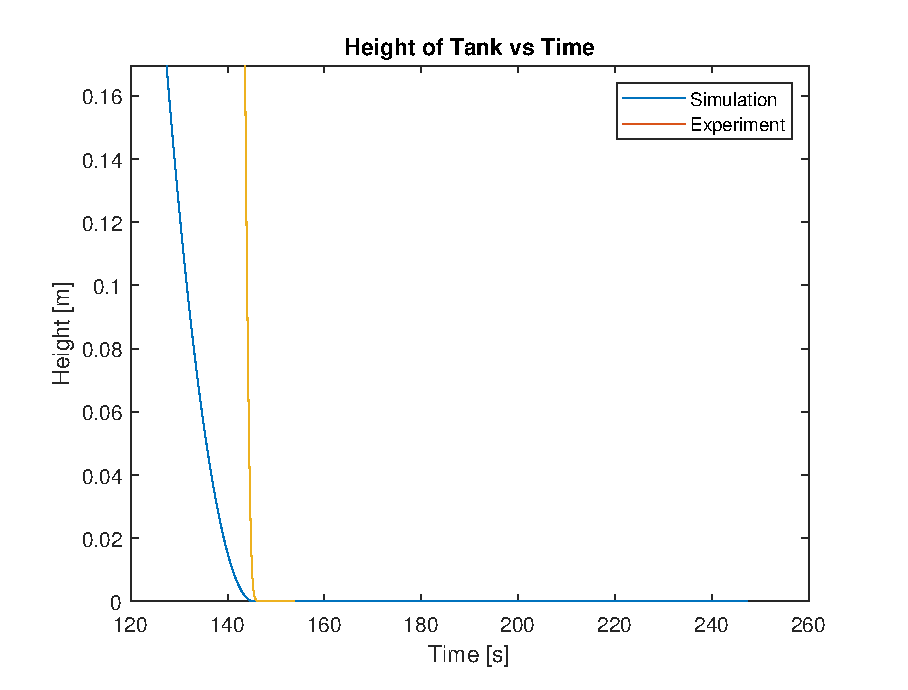
\includegraphics[width = \textwidth]{figures/figure1}
    \caption{Experimental Results and Simulation Results for values of $ C_d. $ The simulation time has been shifted to line up with the experiment. The pump voltage was turned off at around time $ t = 127. $}
    \label{fig:fig1}
  \end{figure}

  \section{Linearity of $ K_p $}

  Using equations (1.2.4) and (1.2.7) we can determine a value for $ K_p. $ If our linear assumption is correct, the value of $ K_p $ will not change based on the pump voltage $ v_p. $ Figure \ref{fig:fig2} shows the results from equation (1.2.4). While it appears that the pump voltage has an effect on the pump coefficient, it only changes by 1E-5 at the most. This change is small enough to still assume that our linear assumption is correct.

  Figure \ref{fig:fig3} shows the results from Equation (1.2.7). We can see that the variation is much smaller at a maximum of .05E-5. This means that the computed values of $ K_p $ are more consistent using Equation (1.2.7) than Equation (1.2.4). We can compute the average value of $ K_p $ found with Equation (1.2.7) for use in future system modeling and control design.

  \begin{equation}
    K_p = 4.4939e-05
  \end{equation}

  \begin{figure}
    \centering
    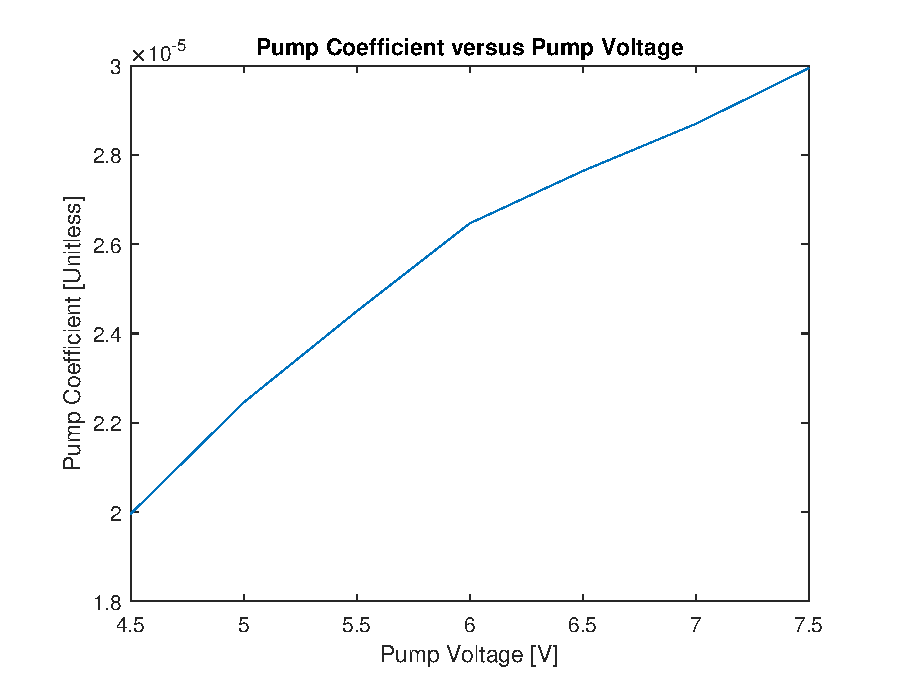
\includegraphics[width=\textwidth]{figures/figure2}
    \caption{Pump Coefficient versus Pump Voltage, $ v_p^{min} = 0 \text { V}. $}
    \label{fig:fig2}
  \end{figure}

  \begin{figure}
    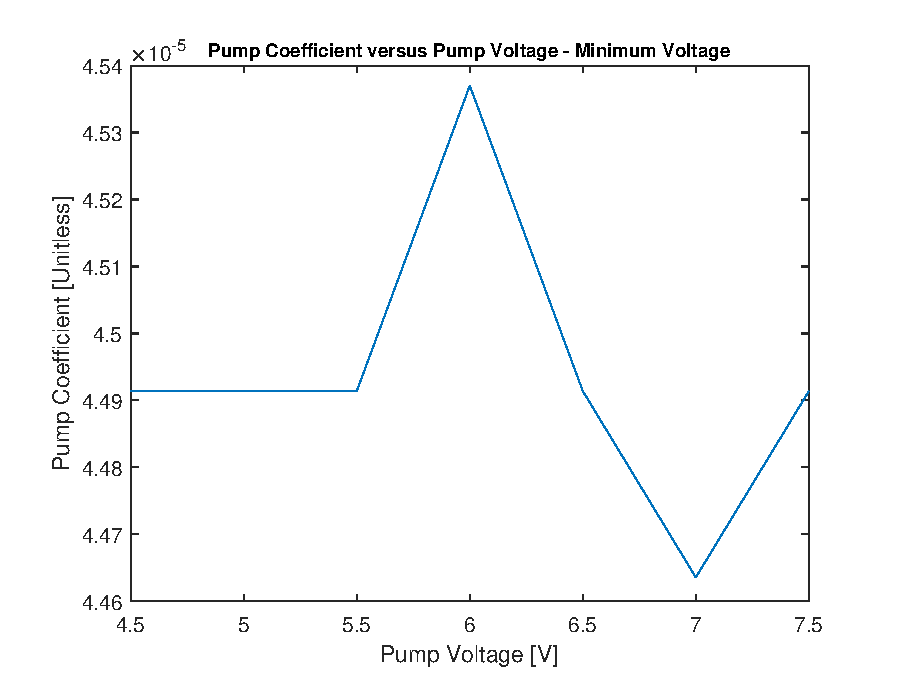
\includegraphics[width=\textwidth]{figures/figure3}
    \caption{Pump Coefficient versus Pump Voltage $ v_p^{min} = 2.5 \text{ V}. $}
    \label{fig:fig3}
  \end{figure}

  \newpage

  \section{Summary}

  One of the key ideas we used is modeling systems with conservation laws. This idea was the basis for determining the mathematical models we used throughout this lab. These models were made assuming that the flow through a resistance is proportional to the pressure across it, the pressure at the bottom of a tank is proportional to the height of the liquid, and that the tank has a constant cross-sectional area.

  \subsection{Part 1}

  In Part 1, we used our mathematical model of configuration 1 to create a simulink model. This model allows us to run simulations and learn how the height changes due to various input. Additionally, the model will help us determine values for both $ C_d $ and $ K_p. $

  \subsection{Part 2}

  In Part 2, we determined the numerical value of $ C_d, $ which represents how quickly the tank drains. We used the Exp\_OpenLoop.mdl to fill up the tank to its steady state height and observe how quickly the water drains. We took note of both the initial height and the time it took for the height to reach 2 cm. Then, we set the initial height value in our model and adjusted the value of $ C_d $ until the model behavior reflected that of the experiment.

  \newpage

  \subsection{Part 3}

  In Part 3, we estimated the value of $ K_p $ with a set of experiments. We chose 5 different values of $ v_p $ and measured the steady state height associated with that value. Table \ref{tab:tab1} shows the steady state height values associated with pump voltage.

  In the prelab, we found an algebraic expression for $ K_p $, assuming steady state operation. We used this expression to calculate and plot an array of $ K_p $ values to see if the pump voltage had an effect on the pump coefficient. If we assumed that the pump had a minimum operating voltage, we could adjust our formula and see if our computed values of $ K_p $ were more accurate.

  \begin{equation}
    K_p = \frac{C_dA_o}{v_p} \sqrt{2gh_1}
  \end{equation}

  \begin{equation}
    K_p = \frac{C_dA_o}{v_p - v_p^{min}} \sqrt{2gh_1}
  \end{equation}

  \begin{table}
    \centering
    \caption{Pump Voltage and Steady State Height}
    \begin{tabular}{c c}
      Voltage (V) & Steady-state height (cm) \\
      \hline
      4.5 & 1.6 \\
      5 & 2.5 \\
      5.5 & 3.6 \\
      6 & 5 \\
      6.5 & 6.4 \\
      7 & 8 \\
      7.5 & 10 \\
    \end{tabular}
    \label{tab:tab1}
  \end{table}




\end{document}
